
\subsection{Definición de ABMs - Clases Admin}%
\label{sub:definición_de_abms_clases_admin}

Para definir un ABM, es decir, una interfaz capaz de manejar el alta, baja y modificación de registros es necesario una entidad. Por este motivo, para obtener
una idea general del funcionamiento de Sonata-Admin, se decidió definir algunas entidades y generar una clase admin\@.
En sonata admin, una clase admin es aquella que, dada una entidad, permite añadir un servicio en la plataforma web sonata que se hace cargo de cada una de estas funciones.

Para crear un admin es necesario extender de la clase \textbf{AbstractAdmin} que provee sonata y, mediante métodos heredados de la misma, configurar la manera en
que se muestra la información\@.
Algunos de estos métodos son:

\begin{itemize}
    \item \textit{configureFormFields:} este método define los campos a mostrarse durante la acción de crear y editar.
    \item \textit{configureListFields:} define los campos a mostrar durante la acción de listar datos.
    \item \textit{configureShowFields:} establece la información a mostrar durante la acción de ver una entrada.
\end{itemize}

\noindent
Además de lo expresado, una clase admin en \textbf{Sonata} permite:
\begin{itemize}
    \item Validar información
    \item Agregar acciones de acuerdo a eventos de cada entidad
    \item Establecer jerarquías entre clases admin
    \item Crear un menú de forma fácil en las vistas del admin
    \item Establecer filtros de búsqueda.
\end{itemize}

Éstas son las funcionalidades que se utilizaron en este proyecto, sin embargo, sonata cuenta aún con más opciones de configuración.

Una clase admin contiene una referencia a la entidad base del mismo a través de un objeto denominado \textbf{subject}, el mismo es utilizado para realizar cada
operación de alta, baja y modificación de la entidad\@.

Para configurar las diferentes secciones del admin, es necesario especificar la información que se desea incluir, esto es posible utilizando el nombre del campo
o un método que otorgue acceso a la propiedad en cuestión\@. Si se desea acceder a asociaciones, (datos que representan la relación de una entidad) se puede hacerlo mediante una notación de puntos, por ejemplo:
si se tiene una instancia de \textbf{Actividad}, la misma tendrá una asociación con una entidad persona\@. Por lo tanto, se puede acceder al nombre de una
persona referenciándola como ``persona.nombre''.
\begin{figure}[h]
    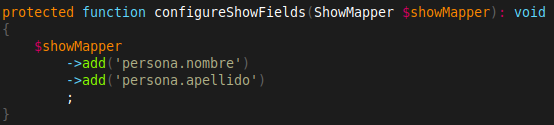
\includegraphics[width=1\linewidth]{image/show.png}
    \caption{Ejemplo de definición de campos a mostrar durante la creación/edición.\newline \textbf{Fuente:} Elaboración propia.}
    \label{fig:image/show}
\end{figure}


\subsubsection{ABMs Compuestas}%
\label{ssub:admin_proyectadmin_proyecto}

En el sistema se separaron las ABM en dos tipos, en primer lugar se tienen aquellas que representan una relacion de 1-n con otros elementos del sistema,
es decir, actividades que pueden relizarse por muchas personas; en segundo lugar están las ABMs de actividades que son realizadas por sólo una persona.


En el primer caso, la implementación se hizo utilizando admins \textit{hijos}, una característica de \textbf{Sonata} que permite definir una jerarquía de clases admin que represente un
elemento \textit{padre} compuesto por uno o muchos elementos \textit{hijos}.

Cuando se asigna un admin como \textit{hijo} se obtienen rutas anidadas, de forma que se puede acceder a acciones del \textit{hijo} desde la vista del padre.
Ej: Una ruta
para acceder a un miembro en particular sería de la forma:\newline \textbf{/miembroproyecto/{id}/(show | edit)}\@.\newline\newline Cuando se accede a los
miembros de cada proyecto se obtienen rutas de la forma:\newline \textbf{/proyecto/{id}/miembroproyecto/{id}/(show | edit)},
\newline \textbf{/proyecto/{id}/miembroproyecto/list}\newline

A continuación se listan las ABM implementadas de esta forma:

\begin{itemize}
        \item Proyecto de Investigación
\item Proyecto de Extensión
\item Rol de Proyectos
\item Comisión de Consejo Superior
\item Práctica Profesional Supervisada
\item Actividad de Divulgación
\item Proyecto de Extensión
\item Curso de Extensión
\item Voluntariado
\item Programa

\end{itemize}

\myparagraph{Implementación de una ABM Compuesta: Proyecto}


En el admin de Proyecto se agregaron los siguientes campos en cada acción:

\begin{itemize}
    \item Lista: nombre del proyecto.
    \item Ver: nombre del proyecto
    \item Inserción: nombre y roles de proyecto.
\end{itemize}

Para asignar un admin como \textit{hijo} se debe configurar el servicio padre a través de un método denominado \textbf{addChild}. Como parámetros requiere el servicio
del admin a actuar de \textit{hijo} y el campo mediante el cual está relacionado al \textit{padre}.


Al agregar un admin como \textit{hijo} se generan las rutas anidadas (sección:~\ref{ssub:admin_proyectadmin_proyecto}), pero no se tiene una forma de acceder a
ellas desde la aplicación web\@. Una buena forma de solucionar este problema es, según la documentación de \textbf{Sonata}, agregar un menú en la barra superior
de la página que contenga botones mediante los cuales acceder a estas rutas.\parencite{sonata-childAdmin}


Para crear un proyecto se deben proporcionar los datos de nombre y roles. Los roles de proyecto están representados en la entidad en forma de Colección,
por lo tanto, se utilizó un tipo de formulario que permite la elección de opciones múltiples y, además, permite agregar nuevas instancias de
rol (figura~\ref{fig:image/proyecto-editar}).

\begin{figure}[h]
    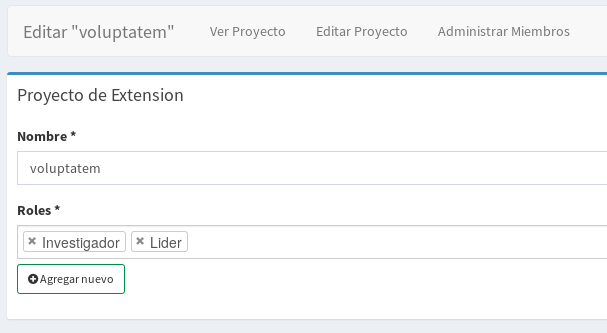
\includegraphics[width=1\linewidth]{image/edit-proyecto.png}
    \caption{Admin: Acción de  editar Proyectos.\newline \textbf{Fuente:} Elaboración propia, captura de pantalla de la aplicación web.}
    \label{fig:image/proyecto-editar}
\end{figure}
\newpage
\myparagraph{Miembro de Proyecto}%

Para la definición del admin de miembros de proyecto se lo estableció como un \textit{hijo} del admin Proyecto, esto es debido a que tiene sentido desde el punto
de vista de la relación que forman. Un proyecto estará integrado por muchos miembros, por lo tanto, al asignar a miembros de proyecto como admin \textit{hijo}
de Proyecto permite administrar los miembros desde la interfaz de proyectos. Al fin y al cabo, la clase admin de miembros no tiene sentido por sí sola.



\begin{figure}[h!]
    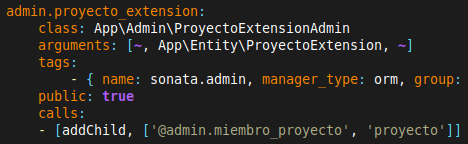
\includegraphics[width=1\linewidth]{image/addChild.png}
    \caption{Servicio admin de Proyecto de Extensión\newline \textbf{Fuente:} Elaboración propia, captura de pantalla de código fuente.}
    \label{fig:image/addChild}
\end{figure}

\myparagraph{Rol de proyecto}%

El admin de roles es muy básico pues solo contiene el campo de nombre. Por lo tanto, en cada una de sus acciones se agregó este único campo.


De igual manera que con \textbf{Proyecto}, se agregó al admin de miembros como \textit{hijo}. De esta forma se puede listar los miembros que cumplen cada rol en
particular.
Esto se logra mediante el método \textbf{addChild} (figura~\ref{fig:image/addChild}) y creando un menú del mismo tipo que el definido en el admin de proyectos.

\subsubsection{ABMs Simples y admins \textit{hijos}}%
\label{ssub:ambs_simples}

En el caso que una actividad solo fuera completada por una persona, o se tratase de un admin \textit{hijo}, la definición del admin solo contendría los
datos de la persona y la actividad\@. Las ABMs implementadas de esta manera se listan a continuación:

\begin{itemize}
        \item Asambleista
\item Consejero Superior
\item Director de Instituto
\item Coordinador de Materia
\item Director de Carrera
\item Miembro de Proyecto
\item Miembro de Comisión de Consejo Superior
\item Miembro de Práctica Profesional Supervisada
\item Rector
\item Miembro de Curso de Extension
\item Miembro de Actividad de Divulgación
\item Miembro de Pasantia
\item Miembro de Voluntariado
\item Responsable de Area
\item Miembro de Programa
\item Vinculador
\item Vice Rector
\item Secretario
\item Beca Befat
\item Movilidad Conurbano Sur
\item Publicacion
\item Movilidad RTF
\item Sub-Secretario

\end{itemize}

\myparagraph{Implementación ABM Simple: Publicación}

Se implementó la entidad extendiendo de la clase \textbf{Actividad} y se definió el admin de manera que:

\begin{itemize}
    \item La acción de crear una publicación requiere especificar la persona, la fecha de inicio y la fecha de fin de la actividad.
    \item Las acciones de listar y visualizar el elemento muestran los datos de la persona y la actividad.
\end{itemize}

Mediante la función \textit{configureFormFields} se establecieron los campos a llenar durante la creación de una Publicación.

\begin{lstlisting}[caption={Definición de campos durante la creación de Publicaciones.\\Fuente: Elaboración propia}]
public function configureFormFields(
    FormMapper $formMapper
): void {
    $formMapper
        ->add('persona', ModelListType::class)
        ->add('inicio', DatePickerType::class)
        ->add('fin', DatePickerType::class)
        ;
}
\end{lstlisting}

Se utilizó un tipo de formulario de \textbf{Sonata} llamado \textbf{ModelListType}, que permite seleccionar las personas a través de una lista y se agregó
un elemento \textbf{Datepicker} para especificar
las fechas\@. Además, se separó la funcionalidad común en un Trait de PHP de manera que si se necesita algo en específico, se puede sobrescribir los métodos
en la clase admin base.
